\begin{frame}<3>{Truncated Linear Congruential Generators}
    \begin{itemize}
            \item Internal state : \(2^k\)-bit state.
            \item Multiplier $a$: known constant.
            \item Initial state: unknown \(2^k\)-bit seed.
    \end{itemize}
    
    \bigskip
    
    \begin{center}
    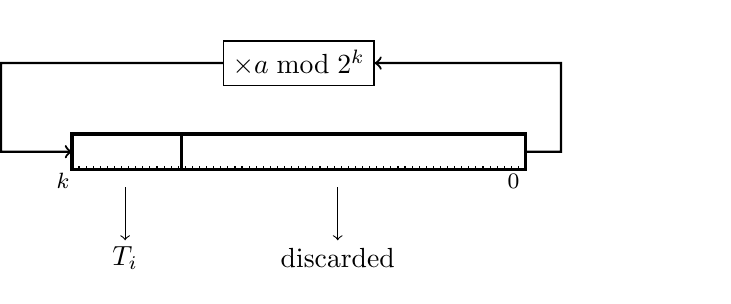
\begin{tikzpicture}[scale=0.45]
      \path[red, use as bounding box] (-1.25, -3) rectangle (17.8, 4);
      
      % S_i
    
        % bordures
        \draw[very thick]  (0, 0) rectangle (12.8, 1);

        \draw<3->[very thick]  (3.1, 0) rectangle +(0, 1);
        \foreach \i in {0, 1, ..., 64} \draw (\i/5, 0) -- +(0, 0.1);
        
        % déco autour
        \node<2->[draw] at (6.4, 3) (update) {$\times a \bmod 2^{k}$};
        \draw<2->[thick,->] (12.8, 0.5) -- (13.8, 0.5) node[below right] {} -- (13.8, 3) -- (update);
%        \draw<2-> (13.7, 2.5) -- +(0.2, -0.2);
%        \path<2-> (13.9, 2.5);
        \draw<2->[thick,->] (update) -- (-2, 3) -- (-2, 0.5) node[below left] {} -- (0, 0.5);
 %       \draw<2-> (-2.1, 2.5) -- +(0.2, -0.2);
%        \path<2-> (-1.9, 2.5);
    
        
        \node[font=\footnotesize,anchor=east] at (12.9, -0.33) {0};
        %\node<3->[font=\footnotesize,anchor=east] at (6.5, -0.33) {64};
        \node[font=\footnotesize] at (-0.25, -0.33) {$k$};
        

        
 
        \draw<3->[->] (1.5, -0.5) -- (1.5, -2);
        \path<3-> (1.7, -1) ;
        \node<3-> at (1.5,-2.5) {\(T_i\)};
        
        \draw<3->[->] (7.5, -0.5) -- (7.5, -2);
        \path<3-> (7.7, -1) ;
        \node<3-> at (7.5,-2.5) {discarded};

      \end{tikzpicture}
    \end{center}
    
\end{frame}

\begin{frame}{Reconstructing Truncated Geometric Sequences}

\begin{itemize}
    \item Sequence $u_{i+1} = a \times u_i \bmod 2^k$.
    \item $T$ = Truncated version (low-order bits unknown).
    %\item Reconstruction algorithm: Frieze \textit{et al} (CVP problem)

\item \(\mathcal{L}\) = lattice spawned by the rows of
\begin{center}
  \begin{tikzpicture}[yscale=0.5]
    \path[red,use as bounding box] (-2, -2.5) rectangle (4.5, 2.5);
    \begin{scope}[yshift=-0.75cm]
    \draw[thick] (-5, 0) rectangle node {$u_i$} +(4, 1);
    \draw[thick,fill=yellow] (-5, -1.5) rectangle node {$T_i$} +(1, 1);
    \draw[thick] (-4, -1.5) rectangle node {?????????} +(3, 1);
  \end{scope}
  
    \node at (1.5, 0) {$\displaystyle
    \begin{pmatrix}
    1 & a   & a^2 & \dots & a^{n-1} \\
    0 & 2^{k} & 0   & \dots & 0 \\
    0 & 0   & 2^{k} & \dots & 0 \\
    \dots & \dots & \dots & \dots & \dots\\
    0 & 0 & 0 & \dots & 2^{k} \\
  \end{pmatrix}$
  };
\end{tikzpicture}
\end{center}
\end{itemize}

\medskip

\begin{block}{Main Idea}
\begin{itemize}
\item $\mathbf{u} = (u_0, u_1, \dots, u_{n-1})$ \textbf{belongs} to the lattice $\mathcal{L}$.
\item $T$ (truncated geometric series) is an \textbf{approximation} of $\mathbf{u}$.
\item[$\Rightarrow$] $T$ is \textbf{close} to a point of $\mathcal{L}$.
\item[$\Rightarrow$] \textbf{Closest} point to $T$ in $\mathcal{L}$ $\leadsto$ $\mathbf{u}$.
\end{itemize}
\end{block}
\end{frame}

%%%%%%%%%%%%%%%%%%%%%%%%%%%%%%%%%%%%%%%%%%%%%%%%

\begin{frame}<1-2>[label=lattice]{\textbf{Lattices and Basis reduction}}
\begin{itemize}
    \item Lattice : subgroup of $\mathbb{R}^n$ isomorphic to $\mathbb{Z}^m$
\end{itemize}
\begin{center}
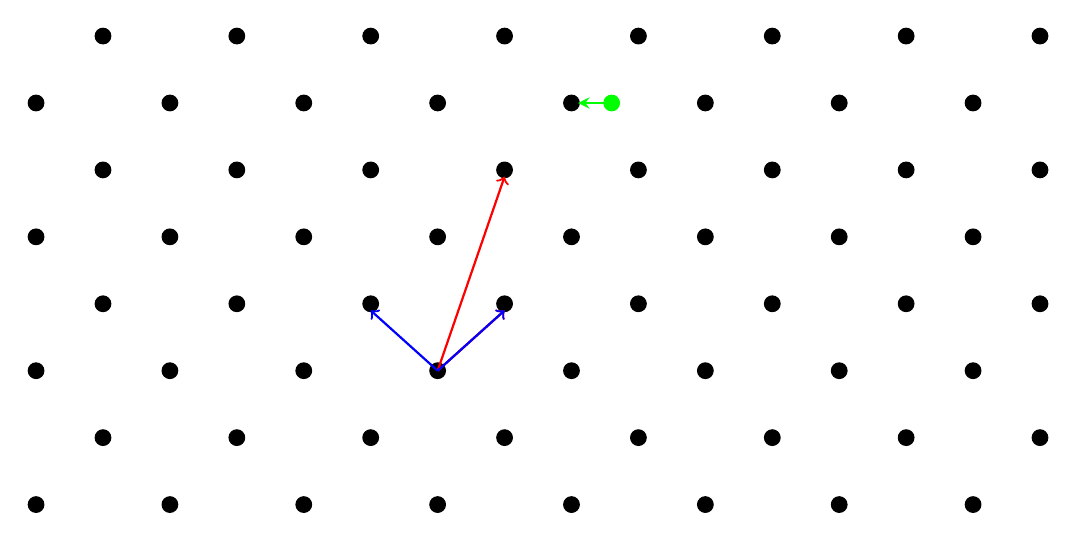
\begin{tikzpicture}[scale=0.85]

    \foreach \x in {0,1,2,3,4,5,6,7}{
		\foreach \y in {-1,0,1,2}{
			\node[draw,circle,inner sep=2pt,fill] at (2*\x,2*\y) {};
			\node[draw,circle,inner sep=2pt,fill] at (2*\x+1,2*\y+1) {};
			
		}
	}
    \draw[->,thick,red] (6,0) --(7,2.9);
    \draw[->,thick,red] (6,0) --(7,0.9);
    
    \draw<3->[->,thick,blue] (6,0) --(7,0.9);
    \draw<3->[->,thick,blue] (6,0) --(5,0.9);
    
    \node<2->[draw,circle,inner sep=2pt,green,fill] at (2*4.3, 2*2) {};
    \draw<2->[draw,thick,green,->,>=stealth] (2*4.3, 2*2) -- +(-0.5, 0);
    
\end{tikzpicture}
\end{center}
% \pause[3]
% \begin{itemize}
%     \item The blue basis is \emph{shorter} than the red basis.
%     \item LLL algorithm reduces bases in polynomial time.
% \end{itemize}
\end{frame}

%%%%%%%%%%%%%%%%%%%%%%%%%%%%%%%%%%%%%%%%%%%%%%%%

\begin{frame}{CVP problem and Babai rounding}
  \begin{alertblock}{Closest Vector Problem}
    \begin{itemize}
    \item Standard \textbf{NP-hard} problem on lattices.
    \item Given arbitrary $\mathbf{x} \in \mathbb{Z}^n$, find closest lattice point.
  \end{itemize}
\end{alertblock}

\medskip

\begin{block}{Babai Rounding Algorithm}
      \begin{itemize}
      \item Approximately solves CVP.
        \[
          BabaiRounding(\mathbf{x}, \mathcal{L}) = H\times \mathrm{round}\left(H^{-1}\times \mathbf{x}\right)
        \]
        Where \(H\) is a ``good'' (LLL-reduced) basis of the lattice $\mathcal{L}$.

      \item FAST (two matrix-vector products + rounding)
      \item Exponentially bad approximation (in the lattice dimension).
      \item[$\rightarrow$] Often exact in small dimension though.
      \end{itemize}
    \end{block}    
\end{frame}

\againframe<2-3>{lattice}


%%% Local Variables:
%%% mode: latex
%%% TeX-master: "../main"
%%% End:
